\documentclass[11pt,a4paper]{article}
\usepackage[margin=2.2cm]{geometry}
\usepackage{amsmath,amssymb}
\usepackage{graphicx}
\usepackage{booktabs,multirow,array,tabularx}
\usepackage{xcolor}
\usepackage{xurl}
\usepackage[hidelinks]{hyperref}
\usepackage{enumitem}
\usepackage{caption}
\usepackage{float}
\captionsetup{font=small,labelfont=bf}
\setlist{itemsep=2pt,topsep=4pt}

\newcommand{\nue}{\ensuremath{\nu_e}}
\newcommand{\numu}{\ensuremath{\nu_\mu}}
\newcommand{\code}[1]{\texttt{\small #1}}
\newcommand{\pend}{{\color{red!70!black}\scriptsize pending}}
\newcolumntype{L}{>{\raggedright\arraybackslash}X}
\newcommand{\tdone}{10}\newcommand{\tplan}{71}

\makeatletter\newcommand{\tabin}[1]{\@@input #1 }\makeatother

\title{\textbf{Charge + Light Foundation Model for MicroBooNE Open Data:\\ Physics-Oriented Metrics and the Light Shortcut}\\[4pt]
\large Technical Note --- Round 4}
\author{Haiwang Yu\thanks{Prepared with the assistance of Claude (Anthropic). Code: \url{https://github.com/HaiwangYu/fm4npp-lartpc}, branch \code{main}, package \code{multi-modal-qlmatch/qlfm}. Tracking: GitHub issue \#6. Rounds 1--3 are described in \code{docs/technote-round\{1,2,3\}.pdf}. The questions studied here were suggested by Xin Qian.}}
\date{October 2026}

\begin{document}
\maketitle

\begin{abstract}
\noindent
Round~4 asks whether the round-2/3 metrics measure what matters for physics. It focuses on four methods: qlfm-M CL (charge + light pretraining), qlfm-M C (the same model pretrained on charge only), Panda (PTv3 + Sonata, charge only) and Pandora. It has four parts:
\begin{enumerate}
  \item \textbf{T1-nu, a per-event $\nu$ hit metric.} The round-3 hit metric (T1) was already $\nu$-only, but it was \emph{pooled} over all hits of all test events. We add per-event completeness, purity and F1 of the $\nu$ hits, as Pandora's own slice metrics are defined.
  \item \textbf{Consistency with Pandora.} We check whether the two are comparable and explain why the event displays do not look as different as the pooled numbers suggest.
  \item \textbf{The light shortcut.} A bright beam-window flash almost implies a $\nu$, so light could make the event-level task (T2) trivial for a model that sees light. We define a large-light cut and re-score T1 and T2 separately on events that pass and fail it.
  \item \textbf{T5, charge$\to$light prediction,} a direct probe of the charge--light correlation. We measure how it scales with pretraining and labelled data.
\end{enumerate}

Findings:
\begin{itemize}
  \item \textbf{Per event, Pandora is much closer to the foundation models than the pooled metric suggests.} Median per-event F1 (charge-weighted): Pandora 0.81, qlfm-M CL 0.91, qlfm-M C 0.80, Panda 0.79. The pooled gap (0.65 vs 0.90) is dominated by the 21\% of events where Pandora's highest-$\nu$-score slice is a cosmic, typically when the $\nu$ carries only a few per cent of the event charge.
  \item \textbf{Light is a strong but not the decisive shortcut for T2.} Beam-window PE alone separates in-AV $\nu$ from no-$\nu$ with AUC 0.93, but only 0.69 among events passing a 200\,PE cut. In that bright subsample qlfm-M CL keeps AUC 0.99, against 0.95--0.97 for Panda, 0.95 for a Pandora + BDT with light, and 0.82--0.86 for qlfm-M C. The advantage comes from charge--light \emph{consistency}, not from flash presence.
  \item \textbf{The light-aware encoder already knows the light.} Predicting the 32-PMT light from charge alone (T5), qlfm-M CL reaches test MSE 0.50 and a 30\% total-PE resolution, against 0.59 / 53\% for qlfm-M C, 0.62 / 67\% for a model trained from scratch, and 0.74 / 87\% for a constant. Its own MAE decoder does as well with no labels at all (0.51 / 33\%). Results saturate at 10\% labels, and beyond about 10\% of the pretraining split, at the current model size and step budget. \tdone{} of \tplan{} runs are complete; the remaining Panda runs are marked pending.
\end{itemize}
\end{abstract}

\tableofcontents
\clearpage

%=====================================================================
\section{Methods compared and data}
%=====================================================================
All numbers use the round-2/3 protocol (R2P): same splits, label pools and test subsets (10k events for T2, 3k for T1). The four methods are:
\begin{itemize}
  \item \textbf{qlfm-M CL} --- 21M multi-modal MAE, charge and light tokens in one transformer, pretrained on 90\% of the pretraining split.
  \item \textbf{qlfm-M C} --- the identical model and pretraining, charge only (\code{--light 0}).
  \item \textbf{Panda} --- PTv3 + Sonata self-distillation on 3D-voxelized hits (charge only).
  \item \textbf{Pandora} --- the MicroBooNE reconstruction in the open-data files. For T1 we use the hits of the slice with the highest \code{nu\_score}. For T2 we use the best \code{nu\_score} directly, and a BDT (HistGradientBoosting) on 32 Pandora charge features, optionally with 8 light features (round~2, Table~2 there).
\end{itemize}
The foundation models are evaluated in the round-3 configurations, from the saved test predictions of those runs; \emph{no model was retrained for parts 1--3}:
\begin{itemize}
  \item XF: frozen backbone + strong late fusion (cross-attention from charge tokens to PMT tokens), the primary configuration;
  \item LL: frozen backbone + the weak round-2 late light;
  \item FT: fine-tuned with round-2 late light;
  \item no light: frozen, without any late light (for qlfm-M CL the light inside the backbone remains).
\end{itemize}
Labels: 1\% or 10\% of the training pool.

%=====================================================================
\section{T1-nu: per-event $\nu$ hit metrics}\label{sec:t1nu}
%=====================================================================
\subsection{Definitions}
A hit is a true $\nu$ hit if the $\nu$ deposited more than 0.05\,MeV in it. A method selects a hit if its $p(\nu)>0.5$; Pandora selects all hits of its $\nu$ slice. With weights $w$ (the hit charge, or 1 for hit counting), for one event:
\[
\text{completeness}=\frac{\sum_{\rm sel\,\cap\,\nu} w}{\sum_{\nu} w},\qquad
\text{purity}=\frac{\sum_{\rm sel\,\cap\,\nu} w}{\sum_{\rm sel} w},\qquad
F1=\frac{2\sum_{\rm sel\,\cap\,\nu} w}{\sum_{\rm sel} w+\sum_{\nu} w}.
\]
\begin{itemize}
  \item \textbf{Pooled} (the round-2/3 T1 metric): the sums run over all hits of all 3{,}000 test events. Large events, and events where a method selects a large cosmic, dominate.
  \item \textbf{Per event} (T1-nu): computed in every event, then summarized by the median and mean over events, and by the fraction of ``good'' events with completeness $>0.5$ and purity $>0.5$. An event where nothing is selected has completeness 0 and F1 0; its purity is undefined and left out of the purity median.
\end{itemize}
Both T1 and T1-nu consider only the $\nu$ class: cosmic hits enter only through the purity. The round-3 T1 was therefore already $\nu$-only; what changes is pooled vs per-event averaging.

\subsection{Results}
\newcommand{\tnuhead}[1]{\toprule
 & & \multicolumn{3}{c}{pooled} & \multicolumn{5}{c}{per event} #1\\
 \cmidrule(lr){3-5}\cmidrule(lr){6-10}
Method & config & eff. & pur. & F1 & comp. & pur. & F1 & F1 & good}
\begin{table}[H]\centering\small
\caption{T1-nu, charge-weighted. Per-event comp., pur.\ and the first F1 are medians; the second F1 is the mean; ``good'' is the fraction of events with comp.\ and pur.\ $>0.5$; ``none'' the fraction where nothing is selected. Pooled F1 is the round-3 T1 metric.}\label{tab:t1nuq}
\setlength{\tabcolsep}{4pt}
\begin{tabular}{llccccccccc}\tnuhead{ & }& none\\
 & & & & & med. & med. & med. & mean & &\\\midrule
\tabin{gen/t1nu_q.tex}
\bottomrule\end{tabular}\end{table}
\begin{table}[H]\centering\small
\caption{T1-nu, hit-count weighted (closest to Pandora's usual hit-based slice metrics). Columns as Table~\ref{tab:t1nuq}.}\label{tab:t1nun}
\setlength{\tabcolsep}{4pt}
\begin{tabular}{llcccccccc}\tnuhead{}\\
 & & & & & med. & med. & med. & mean & \\\midrule
\tabin{gen/t1nu_n.tex}
\bottomrule\end{tabular}\end{table}

\begin{figure}[H]\centering
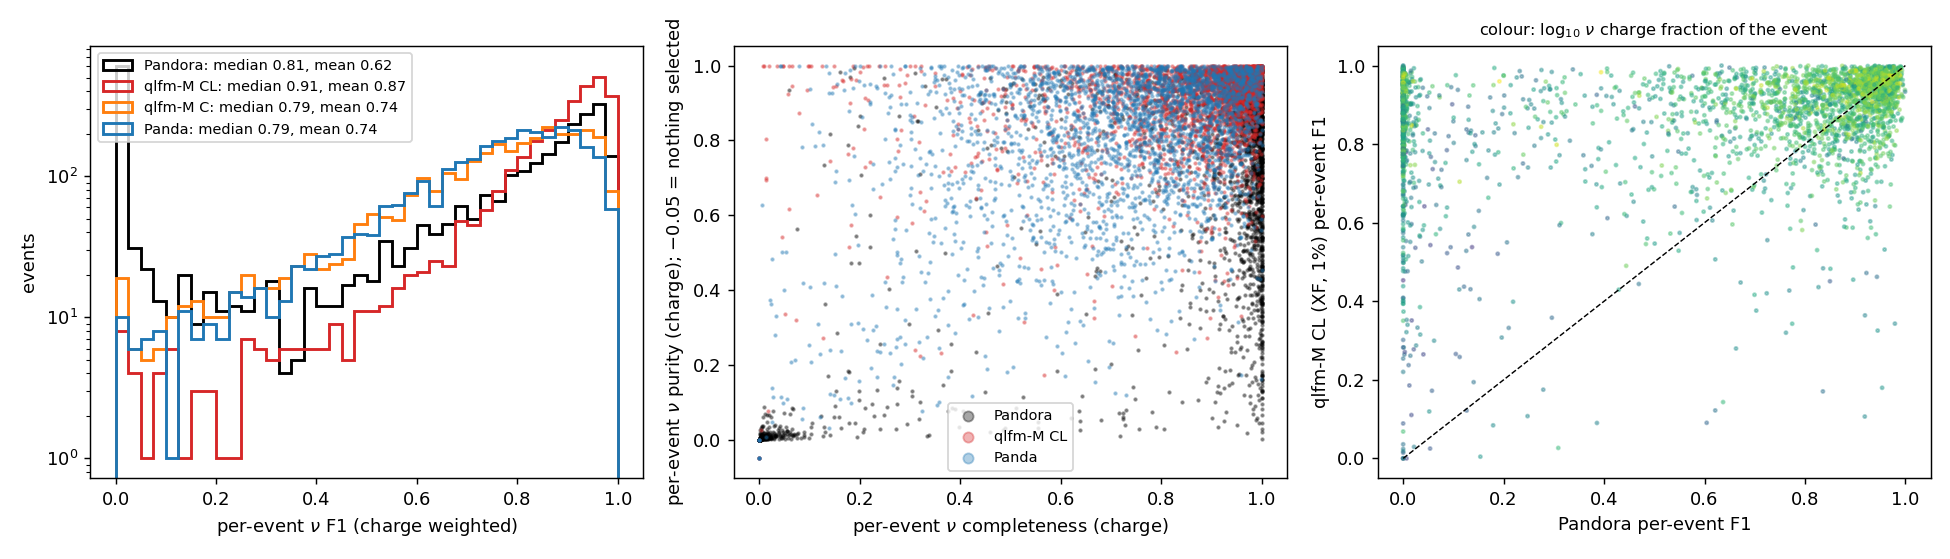
\includegraphics[width=\textwidth]{../figures/round4_t1nu.png}
\caption{T1-nu, charge-weighted, XF 1\% for the models. Left: per-event F1 distributions. Middle: per-event purity vs completeness; points at purity $-0.05$ select nothing. Right: qlfm-M CL vs Pandora per-event F1, coloured by the $\nu$ share of the event charge.}\label{fig:t1nu}
\end{figure}

\paragraph{Reading the tables.}
\begin{itemize}
  \item \textbf{Per event, Pandora is far closer to the models.} Charge-weighted median F1: Pandora 0.807, qlfm-M CL 0.912, qlfm-M C 0.795, Panda 0.787 (XF 1\%). Pooled, the same numbers are 0.651 / 0.899 / 0.792 / 0.792. Pandora gains 0.16 from pooled to per-event median; the models change by at most 0.01.
  \item \textbf{Pandora's profile is high completeness, lower purity.} Median completeness 0.965 is higher than any model's (0.92 for qlfm-M CL), median purity 0.73 lower (0.94). Pandora either finds the whole $\nu$ slice, including cosmic hits merged into it, or misses it entirely; the models make softer, hit-by-hit errors.
  \item \textbf{The mean is pulled down by failures.} Pandora's mean F1 (0.62) is far below its median (0.81) because of a cluster of events at F1 $\approx 0$ (Fig.~\ref{fig:t1nu}, left), and only 64\% of its events are ``good'' vs 94\% for qlfm-M CL.
  \item \textbf{The model ranking is unchanged.} qlfm-M CL $>$ qlfm-M C $\approx$ Panda at 1\% labels with XF; fine-tuning lifts qlfm-M C to 0.925 median, close to qlfm-M CL XF.
\end{itemize}

%=====================================================================
\section{Consistency with Pandora's metrics}\label{sec:pnd}
%=====================================================================
\subsection{Are the definitions the same?}
\begin{itemize}
  \item \textbf{Same in spirit.} Pandora's slice / $\nu$-identification performance is usually quoted per event: completeness and purity of the hits in the selected $\nu$ slice relative to the true $\nu$ hits, by hit count. Our hit-count per-event T1-nu (Table~\ref{tab:t1nun}) follows that definition. The pooled round-3 T1 does not, and should not be compared with Pandora numbers quoted elsewhere.
  \item \textbf{Differences that remain.}
  \begin{itemize}
    \item Our Pandora $\nu$ slice is the slice with the highest \code{nu\_score} in the open-data files. A full MicroBooNE selection also uses the flash-match score and topological cuts and would reject some of the wrong slices below. Our Pandora numbers are therefore a lower bound on what a tuned Pandora-based selection achieves.
    \item Truth matching is per hit with a 0.05\,MeV threshold, rather than via MC-particle back-tracking with shared-hit fractions. Differences arise only for hits shared by $\nu$ and cosmic deposits.
    \item Pandora is scored on the same 3{,}000 test events, including events where the $\nu$ is tiny. Many published numbers are for selected, or for $\nu$ interactions above a size threshold.
  \end{itemize}
\end{itemize}

\subsection{Why the displays do not look very different}
We split the 3{,}000 test events by whether Pandora's slice contains the $\nu$:
\begin{itemize}
  \item \textbf{No slice:} 0\% (Pandora always proposes one).
  \item \textbf{Wrong slice} (it holds $<10\%$ of the $\nu$ charge): \textbf{21\%} of events. The rate grows as the $\nu$'s share of the event charge shrinks: the median share is 3.5\% in wrong-slice events vs 6.2\% otherwise (table below).
  \item \textbf{Right slice} (79\%): Pandora median completeness 0.981, purity 0.824, F1 0.868. On these events the pooled F1 is 0.769 for Pandora and 0.906 for qlfm-M CL.
\end{itemize}
\begin{center}\small
\begin{tabular}{lccccc}\toprule
$\nu$ share of event charge & $<2\%$ & 2--5\% & 5--10\% & 10--20\% & $>20\%$\\\midrule
events & 423 & 946 & 978 & 556 & 97\\
Pandora wrong slice & 38\% & 27\% & 15\% & 11\% & 8\%\\
Pandora median F1$_q$ & 0.13 & 0.72 & 0.84 & 0.91 & 0.92\\
qlfm-M CL median F1$_q$ (XF 1\%) & 0.83 & 0.90 & 0.92 & 0.94 & 0.96\\\bottomrule
\end{tabular}
\end{center}
So the large pooled gap has two sources:
\begin{enumerate}
  \item a failure mode in a fifth of the events, where Pandora selects a cosmic slice and scores 0;
  \item charge weighting, which magnifies cosmic tracks merged into the $\nu$ slice, since a long cosmic muon carries much more charge than a low-energy $\nu$.
\end{enumerate}
On a ``typical'' event both work well (Pandora $\approx$0.8--0.9, qlfm-M CL $\approx$0.9), and the differences are a few stray hits. This is what the round-2 displays mostly showed.

\paragraph{New displays (Appendix~\ref{app:displays}).} We drew 24 events, 6 at random in each of four categories (per-event charge-weighted F1, XF 1\%):
\begin{itemize}
  \item \textbf{Pandora selects a cosmic slice} (436 of 3{,}000 events with qlfm-M CL F1 $>0.8$). Pandora F1 $\approx$0; the models find the small $\nu$ (qlfm-M CL 0.85--0.98, Panda and qlfm-M C 0.61--0.95).
  \item \textbf{Pandora's slice absorbs cosmics} (393 events with Pandora purity $<0.6$ and qlfm-M CL F1 $>0.8$). The $\nu$ slice includes an attached cosmic track, e.g.\ \#5: a 0.38\,GeV \numu CC with 1.5\% of the event charge, where a long cosmic in the slice gives purity 0.15. Charge-only models also struggle here (qlfm-M C 0.55, Panda 0.45), while qlfm-M CL reaches 0.91.
  \item \textbf{Model clearly worse than Pandora} (37 events; Pandora F1 more than 0.25 above qlfm-M CL). In all six the $\nu$ is small (1.8--5\% of the event charge), and the models under-select. E.g.\ \#3, a 0.96\,GeV \nue CC: qlfm-M CL tags only the densest part of the shower (completeness 0.21, purity 0.91), while Pandora's slice gets it all (0.95) but also many scattered hits (purity 0.66).
  \item \textbf{Typical} (both near their median F1). Pandora and qlfm-M CL look alike; the charge-only models occasionally tag pieces of nearby cosmics.
\end{itemize}

%=====================================================================
\section{The light shortcut: a large-light cut}\label{sec:light}
%=====================================================================
\subsection{Light statistics}
The light tokens see all optical hits (ophits) in 0--24\,$\mu$s.
\begin{itemize}
  \item \textbf{Beam window.} The beam flash lies at 3--6\,$\mu$s: the true $\nu$ time spans 3.1--4.7\,$\mu$s, plus a 0.48\,$\mu$s flash lag. We sum the PE of ophits in $[3,6]\,\mu$s per event (\emph{beam-window PE}).
  \item \textbf{Per class} (Fig.~\ref{fig:light}, left), on the T2 test events: most no-$\nu$ events have 20--200\,PE (cosmic light that happens to fall in the window; median $\approx$50\,PE), 79\% of in-AV $\nu$ events have more than 500\,PE, and out-of-AV $\nu$ lie in between.
  \item \textbf{Timing} (Fig.~\ref{fig:light}, middle): the PE-weighted spectrum peaks inside the window for $\nu$ events and is flat for no-$\nu$ events. A long late-light tail exists in all classes.
  \item \textbf{Light alone is a strong T2 discriminant} (in-AV $\nu$ vs no-$\nu$, Fig.~\ref{fig:light}, right): AUC 0.937 for the beam-window PE, 0.906 for the total 0--24\,$\mu$s PE, 0.909 for the largest reconstructed flash.
\end{itemize}

\begin{figure}[H]\centering
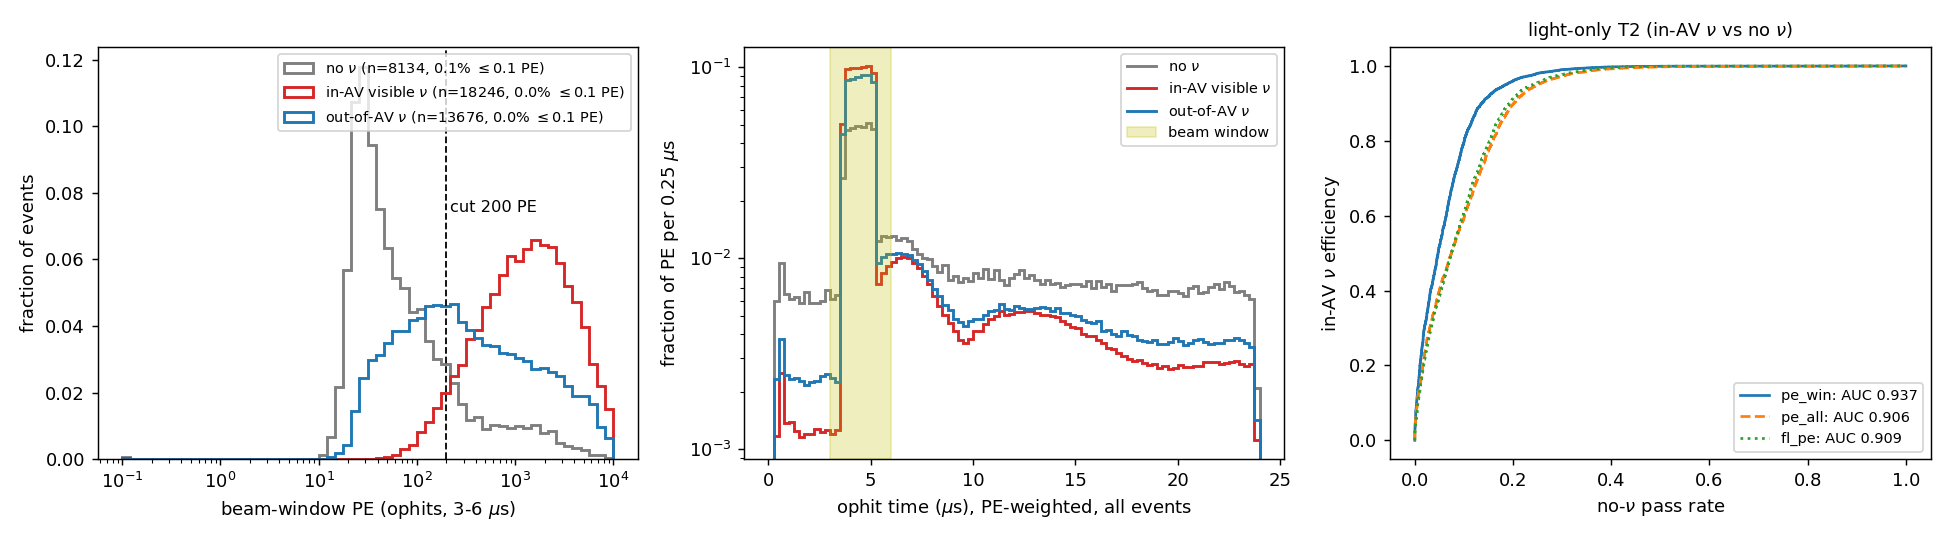
\includegraphics[width=\textwidth]{../figures/round4_light_stats.png}
\caption{Light statistics on the 40{,}056 T2-eligible test events (8{,}134 no-$\nu$, 18{,}246 in-AV, 13{,}676 out-of-AV). Left: beam-window PE per class, with the 200\,PE cut. Middle: PE-weighted ophit time spectrum, beam window shaded. Right: light-only T2 ROC.}\label{fig:light}
\end{figure}

\subsection{The cut}
The balanced accuracy between in-AV $\nu$ and no-$\nu$ is maximal at 218\,PE (0.885). We use a round \textbf{200\,PE in $[3,6]\,\mu$s}:
\begin{center}\small
\begin{tabular}{rccc}\toprule
cut (PE) & in-AV $\nu$ pass & no-$\nu$ pass & out-of-AV $\nu$ pass\\\midrule
50 & 0.999 & 0.492 & 0.880\\
100 & 0.990 & 0.305 & 0.740\\
\textbf{200} & \textbf{0.944} & \textbf{0.177} & \textbf{0.576}\\
500 & 0.790 & 0.099 & 0.383\\\bottomrule
\end{tabular}
\end{center}
Per the request, nothing is retrained: we re-score the saved test predictions separately on events that \emph{pass} and \emph{fail} the cut.
\begin{itemize}
  \item \textbf{pass:} events with a bright beam flash. Here the light no longer tells $\nu$ from no-$\nu$ by itself (light-only AUC 0.69), and the models must use the charge, or the consistency of charge and light.
  \item \textbf{fail:} dim events. A model that relies on ``bright flash $\Rightarrow\nu$'' would lose its $\nu$ efficiency here.
\end{itemize}
Sub-sample sizes: T2 test (no-$\nu$ / in-AV / out-of-AV) all 2026 / 4542 / 3432, pass 385 / 4288 / 1971, fail 1641 / 254 / 1461; T1 test 2{,}834 pass / 166 fail.

\subsection{T2 with and without the cut}
\begin{table}[H]\centering\small
\caption{T2, in-AV $\nu$ vs no-$\nu$ (out-of-AV events excluded): AUC of $p(\text{in-AV})$ on all events, the pass and the fail sub-samples, and in-AV $\nu$ efficiency at 95\% no-$\nu$ rejection (threshold set within each sub-sample). Pandora rows: the best \code{nu\_score} directly, and BDTs on Pandora charge features (C) or charge + light features (C+L), trained on the 1\% or 10\% label pools.}\label{tab:t2cut}
\begin{tabular}{llccccc}\toprule
 & & \multicolumn{3}{c}{AUC} & \multicolumn{2}{c}{eff.\ @ 95\% rej.}\\\cmidrule(lr){3-5}\cmidrule(lr){6-7}
Method & config & all & pass & fail & all & pass\\\midrule
\tabin{gen/t2cut.tex}
\bottomrule\end{tabular}\end{table}
\begin{itemize}
  \item \textbf{The light shortcut is real for simple methods:} light-only AUC drops from 0.930 to 0.693 in the pass sample, and the Pandora direct score is weak everywhere (0.83).
  \item \textbf{qlfm-M CL barely moves:} AUC 0.991--0.996 in the pass sample, efficiency at 95\% rejection 0.98--0.99, for every configuration including ``no late light''. Its encoder has learned which flash belongs to which charge, and uses that rather than the flash brightness.
  \item \textbf{Panda with strong fusion} comes next (0.954 at 1\%, 0.968 at 10\%), level with the Pandora C+L BDT (0.925 / 0.950).
  \item \textbf{qlfm-M C} falls most in the pass sample (0.82--0.86): its late-fusion heads learn mostly the flash brightness. Without late light it reaches only 0.72 overall.
  \item \textbf{Fail sample:} with late light every model keeps a high AUC (0.93--1.00); without it the charge-only models drop (qlfm-M C 0.61, Panda 0.81). Dim events with a $\nu$ are rare (254) and usually small, so here the light shortcut works \emph{against} the $\nu$. qlfm-M CL reaches 0.998--1.000 in every configuration.
\end{itemize}

\subsection{T1 with and without the cut}
\begin{table}[H]\centering\small
\caption{T1 (charge-weighted) on all T1 test events and on the pass / fail sub-samples: pooled F1 and per-event median F1.}\label{tab:t1cut}
\begin{tabular}{llcccccc}\toprule
 & & \multicolumn{2}{c}{all (3000)} & \multicolumn{2}{c}{pass (2834)} & \multicolumn{2}{c}{fail (166)}\\\cmidrule(lr){3-4}\cmidrule(lr){5-6}\cmidrule(lr){7-8}
Method & config & pooled & median & pooled & median & pooled & median\\\midrule
\tabin{gen/t1cut.tex}
\bottomrule\end{tabular}\end{table}
\begin{itemize}
  \item 94\% of T1 events pass the cut, so the pass numbers are essentially the overall ones.
  \item \textbf{Dim events are harder for everyone, but very unequally.} Pandora drops to 0.29 (pooled and median): with a weak flash its slice choice is mostly wrong. qlfm-M CL keeps 0.86 (XF) to 0.91 (FT). Panda drops by 0.09, and qlfm-M C by 0.04 (XF) to 0.16 (no light).
  \item The T1 advantage of qlfm-M CL is therefore not an artefact of bright events; it is largest exactly where the light is weak.
\end{itemize}

%=====================================================================
\section{T5: predicting the light from the charge}\label{sec:t5}
%=====================================================================
\subsection{Task}
T5 measures directly whether an encoder of the TPC charge knows what light the event should produce.
\begin{itemize}
  \item \textbf{Target:} the same light features the qlfm light tokens use. For each of the 32 PMTs: the PE in 16 time bins over 0--24\,$\mu$s (edges 0, 1, 2, 3, 3.5, \dots, 6, 7, 8, 10, 12, 15, 19, 24\,$\mu$s) plus the total, each as $\log(1+\text{PE})$, i.e.\ $32\times17$ numbers per event.
  \item \textbf{Input:} charge only. For qlfm-M CL the light input of the backbone is switched off; no late light is used.
  \item \textbf{Head} (identical for every backbone, trained from labels): 32 learned PMT queries cross-attend for 2 layers to the backbone's charge tokens projected to 256-d, then a linear map to 17 features. About 1.3M parameters.
  \item \textbf{Loss:} MSE over all features + MSE on the total column.
  \item \textbf{Score:} test MSE (10k test events, same subset as T2).
  \item \textbf{Physics summaries} on events with $\geq$200\,PE measured (94\% of events):
  \begin{itemize}
    \item total-PE resolution $\sigma_{\rm tot}$ = half the 16--84\% range of $\Sigma_{\rm pred}/\Sigma_{\rm meas}-1$, and its median (bias);
    \item PMT-pattern distance TV$_{\rm PMT}$ = median of $\frac12\sum_{\rm PMT}|f_{\rm pred}-f_{\rm meas}|$ of the PE fractions;
    \item $\rho$ = correlation of $\log$ total PE over all events.
  \end{itemize}
\end{itemize}

\paragraph{Scaling scan.}
\begin{itemize}
  \item \textbf{Pretraining data:}
  \begin{itemize}
    \item qlfm-S CL / C at 1, 10, 50, 90\% of the pretraining split (existing round-1 checkpoints);
    \item qlfm-M CL / C at 10 and 90\% (qlfm-M C 10\% newly pretrained);
    \item Panda at 10\% (new) and 90\%, same number of iterations.
  \end{itemize}
  \item \textbf{Labelled data:} frozen backbone at 0.1, 1, 10 and 100\% of the training pool (747 to 747k events); fine-tuning of the three 90\% encoders at 1 and 10\%. Batch 32, at most 30 epochs, with a step cap of 6{,}000 at $\leq$1\% labels and 24{,}000 at 10 and 100\% (12{,}000 for fine-tuning at 10\%). A uniform 6{,}000-step cap would let the 10\% and 100\% runs see the same 192k events: in a first pass they reached the same MSE (0.616 vs 0.617 for qlfm-S CL 1\%), i.e.\ the scan would have measured compute rather than data.
  \item \textbf{References:}
  \begin{itemize}
    \item \emph{scratch}: the qlfm-M architecture trained from random initialization;
    \item \emph{zero-shot}: for CL checkpoints, the pretrained MAE decoder predicts the fully masked light tokens from all charge tokens, with no labels at all;
    \item \emph{constant}: the per-PMT, per-feature mean of the test light (MSE 0.736, $\sigma_{\rm tot}=0.87$).
  \end{itemize}
\end{itemize}

\subsection{Results}
\begin{table}[H]\centering\small
\caption{T5 test MSE ($\downarrow$) with a frozen backbone, by pretraining fraction (rows) and labelled fraction (columns). Zero-shot: the CL model's own MAE decoder, no labels.}\label{tab:t5frozen}
\begin{tabular}{llccccc}\toprule
 & & \multicolumn{4}{c}{labelled fraction (frozen)} & \\\cmidrule(lr){3-6}
Encoder & pretrain & 0.1\% & 1\% & 10\% & 100\% & zero-shot\\\midrule
\tabin{gen/t5_frozen.tex}
\bottomrule\end{tabular}\end{table}
\begin{table}[H]\centering\small
\caption{T5 physics summaries for the round-4 encoders (90\% pretraining). $\sigma_{\rm tot}$, bias and TV$_{\rm PMT}$ on events with $\geq$200\,PE; $\rho$ on all events.}\label{tab:t5phys}
\begin{tabular}{lllccccc}\toprule
Encoder & mode & labels & MSE & $\sigma_{\rm tot}$ & bias & TV$_{\rm PMT}$ & $\rho$\\\midrule
\tabin{gen/t5_physics.tex}
\bottomrule\end{tabular}\end{table}
\begin{figure}[H]\centering
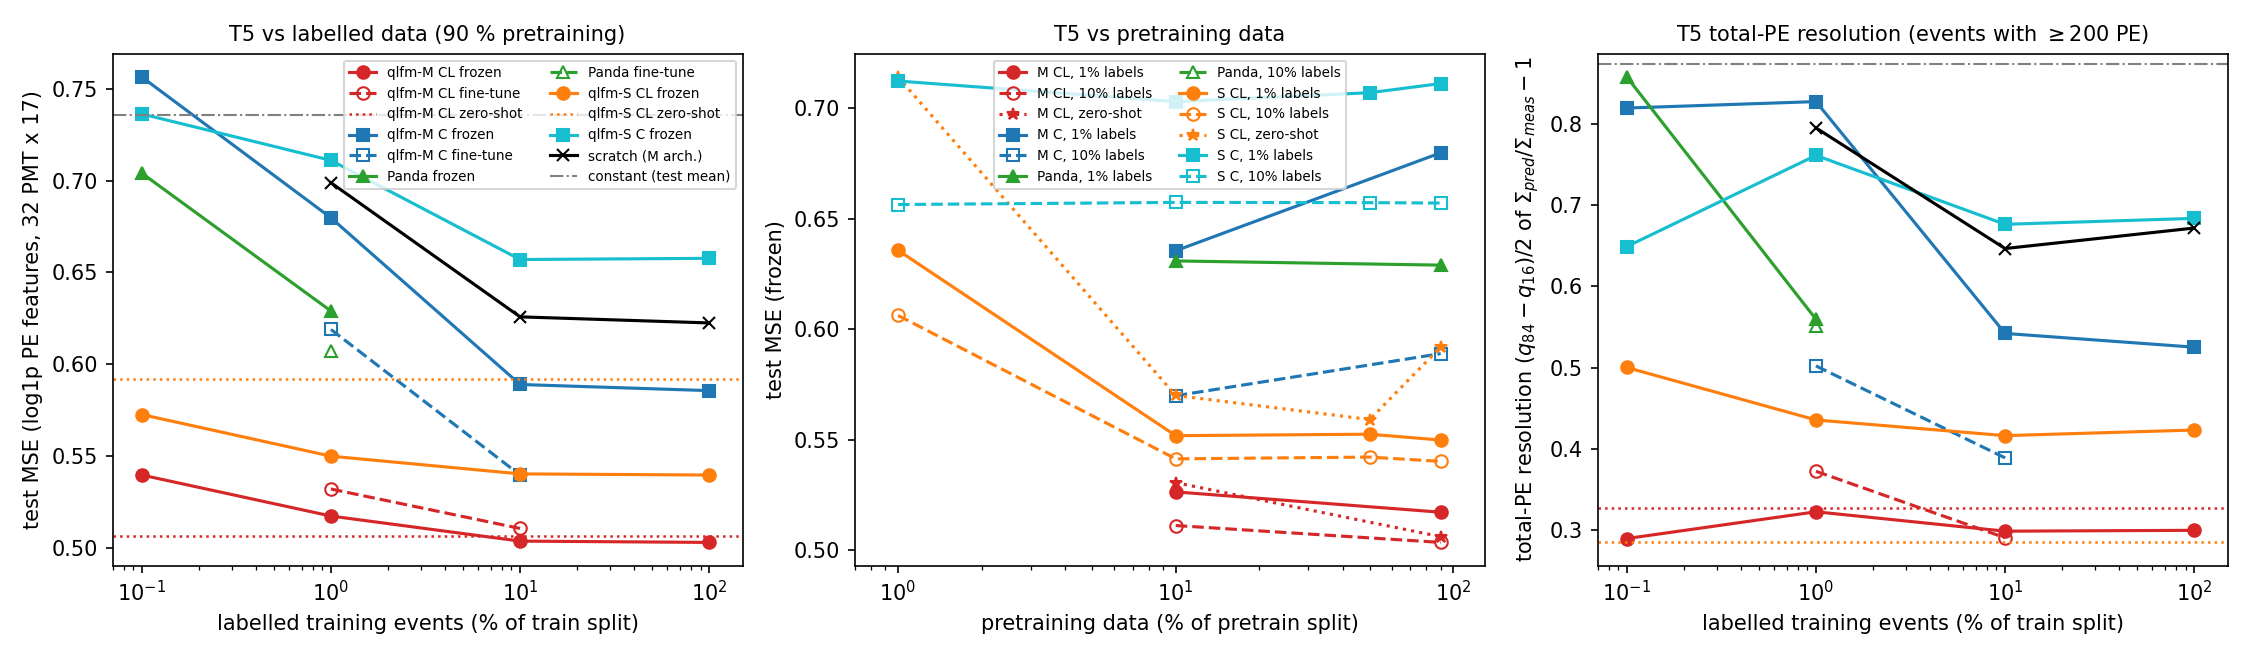
\includegraphics[width=\textwidth]{../figures/round4_t5_scaling.png}
\caption{T5 scaling. Left: test MSE vs labelled data (90\% pretraining; dotted lines: zero-shot). Middle: MSE vs pretraining data, frozen at 1\% and 10\% labels. Right: total-PE resolution vs labelled data.}\label{fig:t5}
\end{figure}

\subsection{Discussion}
\paragraph{Light in pretraining is what matters.} For every model size and every labelled fraction, encoders pretrained with light predict it far better than the same encoders pretrained on charge only:
\begin{itemize}
  \item frozen, 100\% labels: qlfm-M CL 0.503, qlfm-M C 0.586, scratch 0.622, constant 0.736;
  \item total-PE resolution $\sigma_{\rm tot}$: 0.30 (M CL), 0.53 (M C), 0.67 (scratch), 0.87 (constant);
  \item PMT pattern TV$_{\rm PMT}$: 0.16, 0.26, 0.31, 0.44.
\end{itemize}
The same ordering holds at the small size (qlfm-S CL 0.540 vs S C 0.658 at 100\% labels). The charge-only encoders still beat scratch, so the charge MAE learns something about the light yield, but most of the gap is only closed when the pretraining sees the light. Fine-tuning qlfm-M C at 10\% labels (0.540, $\sigma_{\rm tot}$ 0.39) closes about 60\% of its frozen gap to qlfm-M CL, but does not reach it.

\paragraph{The CL model needs no labels.} The zero-shot qlfm-M CL (its own MAE decoder, all light masked) reaches MSE 0.506 and $\sigma_{\rm tot}=0.33$, i.e.\ within 0.003 in MSE of the best labelled frozen result. Labels add almost nothing for this encoder; fine-tuning at 1\% labels is even slightly worse (0.532) than leaving the backbone frozen. This is the direct counterpart of the T2 light-cut result (Sec.~\ref{sec:light}): the CL backbone carries an internal prediction of the light from the charge, which is what lets it check charge--light \emph{consistency} in bright events.

\paragraph{Scaling with labelled data.} All frozen encoders improve steeply from 0.1\% to 10\% labels and are flat from 10\% to 100\% (change $\leq$0.008 in MSE). Scratch is flat too (0.626 vs 0.622). This flatness should not be read as saturation in data: with the 24{,}000-step cap, 100\% labels is about one epoch (768k of 747k events) against about ten epochs at 10\%, so the two points have the same compute. The scan shows that 10\% of the labels is enough for a 1.3M-parameter head at this compute; whether more steps would let 100\% pull ahead is not tested.

\paragraph{Scaling with pretraining data.}
\begin{itemize}
  \item qlfm-S CL: a large step from 1\% to 10\% of the pretraining split (0.636 $\to$ 0.552 at 1\% labels), then flat up to 90\%.
  \item qlfm-S C: flat at every fraction (0.70--0.71 at 1\% labels).
  \item qlfm-M CL: a small gain from 10\% to 90\% (0.526 $\to$ 0.517 at 1\% labels; zero-shot 0.531 $\to$ 0.506).
  \item qlfm-M C: the 10\% checkpoint is \emph{better} than the 90\% one (0.635 vs 0.680 at 1\% labels, 0.567 vs 0.586 at 100\%). Its pretraining validation loss is also lower (0.321 vs 0.333 after the same 34{,}000 steps).
  \item Panda: 10\% and 90\% are equal at every labelled fraction (0.631 vs 0.629 at 1\%, 0.576 vs 0.577 at 100\%).
\end{itemize}
All pretraining runs at a given size use the same number of steps, so the larger fractions see each event fewer times; beyond about 10\% of the split the pretraining is limited by steps and model size, not by data. The one clear data effect is that light-aware pretraining on only 1\% of the split is not enough. A real data-scaling study needs the step count (and model size) to grow with the data.

\paragraph{Charge-only encoders: qlfm-M C vs Panda.} At 1\% labels Panda is better than qlfm-M C, frozen (0.629 vs 0.680; $\sigma_{\rm tot}$ 0.56 vs 0.83) and fine-tuned (0.607 vs 0.619). With more labels the two converge. Frozen, Panda stays slightly ahead (0.580 vs 0.589 at 10\%, 0.577 vs 0.586 at 100\%; $\sigma_{\rm tot}$ 0.51 vs 0.53). Fine-tuned at 10\%, qlfm-M C is ahead (0.540 vs 0.557; $\sigma_{\rm tot}$ 0.39 vs 0.43). Neither charge-only encoder approaches the light-aware one (0.503 frozen, 0.506 zero-shot).

\paragraph{All models under-predict the total light.} The median bias of $\Sigma_{\rm pred}/\Sigma_{\rm meas}-1$ is negative for every model ($-0.07$ for qlfm-M CL, $-0.24$ for qlfm-M C frozen, $-0.52$ for the constant). Part of this is the loss: regressing $\log(1+\text{PE})$ per bin predicts something closer to a geometric mean, and the sum of exponentiated bin predictions is then low. Correcting it would need a loss on linear PE or a calibration; it does not affect the comparison between encoders.


%=====================================================================
\section{Limitations}
%=====================================================================
\begin{itemize}[leftmargin=*]
\item Our Pandora $\nu$ slice ignores the flash-match score and the selection cuts of a real analysis; a tuned selection would recover part of the 21\% wrong-slice events.
\item The light cut is applied at test time only. Training on bright events only (or with light randomly dropped) would test how much of each model's T2 skill \emph{depends} on light; this is not done here.
\item T5 uses a single seed and one head design. The zero-shot point uses the MAE decoder at a different masking ratio (all light masked) than in pretraining.
\item The T5 constant reference uses the test-set mean and is thus slightly optimistic.
\item The T5 scaling scans keep the step count fixed per point: the pretraining runs use the same steps at every data fraction, and 10\% and 100\% labels get the same 24{,}000 steps. Both axes therefore saturate partly because of compute, not data.
\end{itemize}

%=====================================================================
\section{Reproducibility and compute}
%=====================================================================
\sloppy
\begin{itemize}[leftmargin=*]
\item Parts 1--3 (CPU only, from saved predictions):
  \begin{itemize}
    \item \code{scripts/r4\_light\_stats.py} --- light statistics and cut;
    \item \code{scripts/r4\_posthoc.py} --- T1-nu, Pandora consistency, cut sub-samples, display selection;
    \item \code{scripts/r4\_event\_displays.py} --- the 24 displays.
  \end{itemize}
\item T5:
  \begin{itemize}
    \item \code{qlfm/models/heads.py} (\code{LightHead}), \code{qlfm/train\_downstream.py --task light}, \code{qlfm/evaluate.py} (\code{light\_metrics});
    \item \code{qlfm/t5\_zeroshot.py} --- MAE zero-shot;
    \item \code{scripts/make\_tasks\_r4.py} --- the run list, run by \code{scripts/run\_queue.sh};
    \item \code{scripts/summarize\_r4\_t5.py} --- tables and figure.
  \end{itemize}
\item New pretraining: qlfm-M C on 10\% (\code{qlfm.pretrain}, round-3 recipe, \code{--light 0}); Panda on 10\% (\code{qlfm/ref/pimm\_configs/panda\_uboone\_f010.py}; the dataset cycles the smaller subset to keep 28{,}750 iterations).
\item Compute: round~4 used 24.53 node-hours (\code{docs/figures/round4\_node\_hours.md}); 3.7 of them for the Panda 10\% pretraining on the debug-scaling queue, the rest for 2-node bundles (one node: qlfm-M C 10\% pretraining, then T5 runs; the other: T5 runs). Parts 1--3 used no GPU time.

\end{itemize}

\appendix
%=====================================================================
\section{Event displays}\label{app:displays}
%=====================================================================
Each page shows one test event:
\begin{itemize}
  \item the TPC charge (hit integral) in the three planes;
  \item the PMT view of the flash matched to the true $\nu$ time (round-2 Appendix);
  \item the truth, Pandora's $\nu$ slice, and qlfm-M CL, qlfm-M C and Panda (frozen + XF, 1\% labels; colour $=p(\nu)$);
  \item a box with each method's per-event completeness / purity / F1, charge- and hit-count weighted.
\end{itemize}
Dashed boxes mark the 1--99\% extent of the true $\nu$ hits per plane. Order: Pandora selects a cosmic slice (\#1--6), Pandora's slice absorbs cosmics (\#1--6), model worse than Pandora (\#1--6), typical (\#1--6).
\clearpage
\begin{center}\includegraphics[height=0.86\textheight,width=\textwidth,keepaspectratio]{displays/pnd_wrong_slice01.png}\end{center}\clearpage
\begin{center}\includegraphics[height=0.86\textheight,width=\textwidth,keepaspectratio]{displays/pnd_wrong_slice02.png}\end{center}\clearpage
\begin{center}\includegraphics[height=0.86\textheight,width=\textwidth,keepaspectratio]{displays/pnd_wrong_slice03.png}\end{center}\clearpage
\begin{center}\includegraphics[height=0.86\textheight,width=\textwidth,keepaspectratio]{displays/pnd_wrong_slice04.png}\end{center}\clearpage
\begin{center}\includegraphics[height=0.86\textheight,width=\textwidth,keepaspectratio]{displays/pnd_wrong_slice05.png}\end{center}\clearpage
\begin{center}\includegraphics[height=0.86\textheight,width=\textwidth,keepaspectratio]{displays/pnd_wrong_slice06.png}\end{center}\clearpage
\begin{center}\includegraphics[height=0.86\textheight,width=\textwidth,keepaspectratio]{displays/pnd_low_purity01.png}\end{center}\clearpage
\begin{center}\includegraphics[height=0.86\textheight,width=\textwidth,keepaspectratio]{displays/pnd_low_purity02.png}\end{center}\clearpage
\begin{center}\includegraphics[height=0.86\textheight,width=\textwidth,keepaspectratio]{displays/pnd_low_purity03.png}\end{center}\clearpage
\begin{center}\includegraphics[height=0.86\textheight,width=\textwidth,keepaspectratio]{displays/pnd_low_purity04.png}\end{center}\clearpage
\begin{center}\includegraphics[height=0.86\textheight,width=\textwidth,keepaspectratio]{displays/pnd_low_purity05.png}\end{center}\clearpage
\begin{center}\includegraphics[height=0.86\textheight,width=\textwidth,keepaspectratio]{displays/pnd_low_purity06.png}\end{center}\clearpage
\begin{center}\includegraphics[height=0.86\textheight,width=\textwidth,keepaspectratio]{displays/model_worse01.png}\end{center}\clearpage
\begin{center}\includegraphics[height=0.86\textheight,width=\textwidth,keepaspectratio]{displays/model_worse02.png}\end{center}\clearpage
\begin{center}\includegraphics[height=0.86\textheight,width=\textwidth,keepaspectratio]{displays/model_worse03.png}\end{center}\clearpage
\begin{center}\includegraphics[height=0.86\textheight,width=\textwidth,keepaspectratio]{displays/model_worse04.png}\end{center}\clearpage
\begin{center}\includegraphics[height=0.86\textheight,width=\textwidth,keepaspectratio]{displays/model_worse05.png}\end{center}\clearpage
\begin{center}\includegraphics[height=0.86\textheight,width=\textwidth,keepaspectratio]{displays/model_worse06.png}\end{center}\clearpage
\begin{center}\includegraphics[height=0.86\textheight,width=\textwidth,keepaspectratio]{displays/typical01.png}\end{center}\clearpage
\begin{center}\includegraphics[height=0.86\textheight,width=\textwidth,keepaspectratio]{displays/typical02.png}\end{center}\clearpage
\begin{center}\includegraphics[height=0.86\textheight,width=\textwidth,keepaspectratio]{displays/typical03.png}\end{center}\clearpage
\begin{center}\includegraphics[height=0.86\textheight,width=\textwidth,keepaspectratio]{displays/typical04.png}\end{center}\clearpage
\begin{center}\includegraphics[height=0.86\textheight,width=\textwidth,keepaspectratio]{displays/typical05.png}\end{center}\clearpage
\begin{center}\includegraphics[height=0.86\textheight,width=\textwidth,keepaspectratio]{displays/typical06.png}\end{center}\clearpage


\end{document}
